%\documentclass[a4paper]{article}
\usepackage[utf8]{inputenc}
\usepackage[spanish, es-tabla, es-noshorthands]{babel}
\usepackage[table,xcdraw]{xcolor}
\usepackage[a4paper, footnotesep = 1cm, width=22cm, top=2.5cm, height=25cm, textwidth=20cm, textheight=25cm]{geometry}
%\geometry{showframe}

\usepackage{tikz}
\usepackage{amsmath}
\usepackage{amsfonts}
\usepackage{amssymb}
\usepackage{float}
\usepackage{graphicx}
\usepackage{caption}
\usepackage{subcaption}
\usepackage{multicol}
\usepackage{multirow}
\usepackage{wrapfig}
\setlength{\doublerulesep}{\arrayrulewidth}
\usepackage{booktabs}

\usepackage{hyperref}
\hypersetup{
    colorlinks=true,
    linkcolor=blue,
    filecolor=magenta,      
    urlcolor=blue,
    citecolor=blue,    
}

\newcommand{\note}[1]{
	\begin{center}
		\huge{ \textcolor{red}{#1} }
	\end{center}
}

\setcounter{topnumber}{2}
\setcounter{bottomnumber}{2}
\setcounter{totalnumber}{4}
\renewcommand{\topfraction}{0.85}
\renewcommand{\bottomfraction}{0.85}
\renewcommand{\textfraction}{0.15}
\renewcommand{\floatpagefraction}{0.8}
\renewcommand{\textfraction}{0.1}
\setlength{\floatsep}{5pt plus 2pt minus 2pt}
\setlength{\textfloatsep}{5pt plus 2pt minus 2pt}
\setlength{\intextsep}{5pt plus 2pt minus 2pt}

\newcommand{\quotes}[1]{``#1''}
\usepackage{array}
\newcolumntype{C}[1]{>{\centering\let\newline\\\arraybackslash\hspace{0pt}}m{#1}}
\usepackage[american]{circuitikz}
\usetikzlibrary{calc}
\usepackage{fancyhdr}
\usepackage{units} 

\graphicspath{{../Ejercicio-1/}{../Ejercicio-2/}{../Ejercicio-3/}{../Ejercicio-4/}{../ParteI/}{../ParteII/}{../ParteIII/}{../ParteIV/}}

\pagestyle{fancy}
\fancyhf{}
\lhead{22.14 - Electrónica IV}
\rhead{Mechoulam, Lambertucci, Londero}
\rfoot{Página \thepage}


%\begin{document}

\subsection{Introducción}

Se analizó la conmutación de un MOSFET \href{https://www.vishay.com/docs/91019/91019.pdf}{IRF530} de potencia en un circuito con carga inductiva, utilizando un diodo \href{https://www.onsemi.com/pdf/datasheet/mur420-d.pdf}{MUR460} de potencia para proporcionar un camino a la corriente durante el apagado del MOSFET y no dañar al circuito.

%Aca puede ir la foto del circuito

Para la conmutación del MOSFET se utilizó un periodo de $T_s = 16.67 \mu s$ y un duty cycle de $D = 50 \%$.

\subsection{Circuito en la Teoría}

En la teoría, se consideró al diodo MUR460 como ideal excepto por la caída de potencial de la juntura en directa, siendo esta extraída de la datasheet, con un valor de $V_{D_{on}} = 1.3V$. Además, se consideró a la bobina con resistencia serie.

\begin{figure}[H]
	\centering
	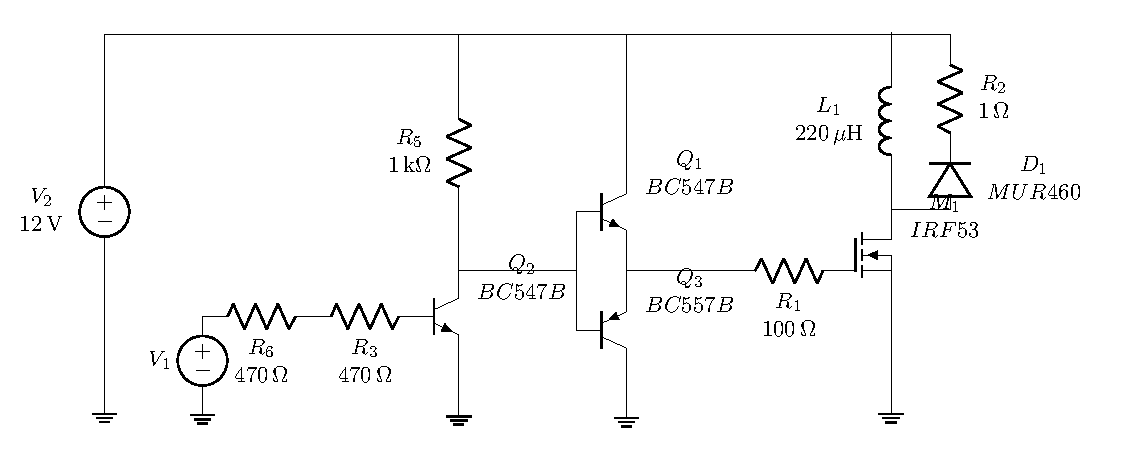
\includegraphics[width=0.7\linewidth, page=1]{ImagenesEjercicio-1/CircuitsEj1}
	\caption{Circuito para el estudio de la conmutación del MOSFET.}
	\label{ej1:fig:circuito}
\end{figure}

\subsubsection{Primer Hemicircuito: MOSFET ON}

Cuando el MOSFET se encuentra encendido, se forma un circuito RL entre la bobina y la $R_{ds_{on}}$ del MOSFET. Como el diodo se encuentra con su ánodo conectado a aproximadamente tierra, y su cátodo conectado a $V_i$, este se encuentra en inversa por lo que no circula corriente a través de él.

\begin{figure}[H]
	\centering
	\includegraphics[width=0.4\linewidth, page=3]{ImagenesEjercicio-1/CircuitsEj1}
	\caption{Hemicircuito con MOSFET encendido.}
	\label{ej1:fig:circuito_on}
\end{figure}

Resolviendo el circuito RL, se puede observar en las ecuaciones (\ref{ej1:eq:IL_on}) y (\ref{ej1:eq:VL_on}) que durante el MOSFET se encuentra encendido aumenta la energía almacenada en la bobina. Sobre el MOSFET caen $V_{ds_{on}} = I_{L_{on}}\cdot R_{ds_{on}}$

\begin{equation}
	 I_{L_{on}}(t) = \left( \left. I_{L_{off}} \right|_{t= n/f_{sw}} -\frac{V_2}{R_{ds_{on}}+R_2}\right) e^{-\frac{R_{ds_{on}}+R_2}{L}t} + \frac{V_2}{R_{ds_{on}}+R_2} \ \ \ \ n \in \mathbb{N}
\label{ej1:eq:IL_on}
\end{equation}

\begin{equation}
	V_{L_{on}}(t) = \left( V_2 - \left. I_{L_{off}} \right|_{t= n/f_{sw}}\cdot (R_{ds_{on}}+R_2) \right)e^{-\frac{R_{ds_{on}}+R_2}{L}t} \ \ \ \ n \in \mathbb{N}
\label{ej1:eq:VL_on}
\end{equation}

Donde $t=\frac{n}{f_{sw}}$ son los momentos en los que el MOSFET conmuta de apagado a encendido y $\left. I_{L_{off}} \right|_{t= n/f_{sw}}$ la corriente en la bobina en dicho momento.

\subsubsection{Segundo Hemicircuito: MOSFET OFF}

Una vez apagado el MOSFET, la bobina posee la tensión $V_{L_{off}}$ necesaria entre sus bornes para que siga circulando la corriente $I_{L_on}$. Sobre el MOSFET caen $V_{ds_{off}} = V_2 + V_D = 13.3V$ circulando la malla formada por el diodo, el MOSFET y la fuente de entrada. En este estado, si se desprecia la corriente parásita del MOSFET, toda la corriente $I_{L_{off}}$ de la bobina pasa por el diodo el cual se encuentra polarizado en directa a consecuencia de la tensión impuesta por la bobina y no se extrae corriente de la fuente de alimentación.

\begin{figure}[H]
	\centering
	\includegraphics[width=0.4\linewidth, page=2]{ImagenesEjercicio-1/CircuitsEj1}
	\caption{Hemicircuito con MOSFET apagado.}
	\label{ej1:fig:circuito_off}
\end{figure}

Resolviendo el circuito RL que se obtiene en este estado, se observa que la bobina tiene una pérdida de energía almacenada dada por las ecuaciones (\ref{ej1:eq:IL_off}) y (\ref{ej1:eq:VL_off}).

\begin{equation}
	 I_{L_{off}}(t) = \left( \left. I_{L_{on}} \right|_{t= nD/f_{sw}} -\frac{V_d}{R_2}\right) e^{-\frac{R_2}{L}t} + \frac{V_d}{R_2} \ \ \ \ n \in \mathbb{N}_o
\label{ej1:eq:IL_off}
\end{equation}

\begin{equation}
	 V_{L_{off}}(t) = \left( V_d - \left. I_{L_{on}} \right|_{t= nD/f_{sw}} \cdot R_2 \right)e^{-\frac{R_2}{L}t} \ \ \ \ n \in \mathbb{N}_o
\label{ej1:eq:VL_off}
\end{equation}

Donde $t=\frac{nD}{f_{sw}}$ son los momentos en los que el MOSFET conmuta de encendido a apagado y $\left. I_{L_{on}} \right|_{t= nD/f_{sw}}$ la corriente en la bobina en dicho momentos. 

\subsubsection{Análisis en Estado Permanente}

En electrónica, se define el estado permanente de un circuito como la condición en la cual los efectos transitorios ya no son importantes. Para el circuito en cuestión, tiempo variante con dos estados específicos, se llega al estado permanente cuando las señales del circuito se tornan completamente periódicas según el periodo de conmutación. 

Analizando la constante de tiempo $\frac{L}{R} = 189.65\mu s$ de los hemicircuitos conformados por la carga inductiva, se observa que ésta es una orden de magnitud mayor que el tiempo que se transcurre en cada estado $t_{on} = t_{off} = \frac{D}{f_{sw}} = \frac{0.5}{60kHz} = 8.33\mu s$ por lo que se puede aproximar la tensión $V_L$ en cada estado como constante y la corriente $I_L$ como rectas de pendiente $\frac{V_L}{L}$. Para hallar la corriente media $\bar{I_L}$ de la bobina se realiza el promedio ponderado por el duty cycle de conmutación de los estados permanentes de ambos hemicircuitos, quedando

\begin{equation}
	\bar{I_L} = \left. I_{L_{on}}\right|_{t \rightarrow \infty} \cdot D + \left. I_{L_{off}}\right|_{t \rightarrow \infty} \cdot (1-D) = \frac{12V}{1\Omega + 0.16\Omega} \cdot 0.5 + 0V \cdot (1-0.5) = 5.17A
\label{ej1:eq:ilbar}
\end{equation}

Esto puede también resolverse de manera gráfica considerando las Ecuaciones (\ref{ej1:eq:IL_on}) y (\ref{ej1:eq:IL_off}) de las corrientes de la bobina para cada hemicircuito. En la Figura (\ref{ej1:fig:ILmediagrafico}) se observa que el cruce de ambas envolventes será la solución para la corriente media en la bobina en régimen permanente de conmutación. Tener en cuenta que la Ecuación (\ref{ej1:eq:IL_off}) supone al diodo como una fuente de tensión constante que no se apaga aunque la corriente sea cero. Debido a esto, no se tuvo en cuenta de la Ecuación (\ref{ej1:eq:IL_off}) la solución particular de la ecuación diferencial para el gráfico de la Figura (\ref{ej1:fig:ILmediagrafico}).

\begin{figure}[H]
	\centering
	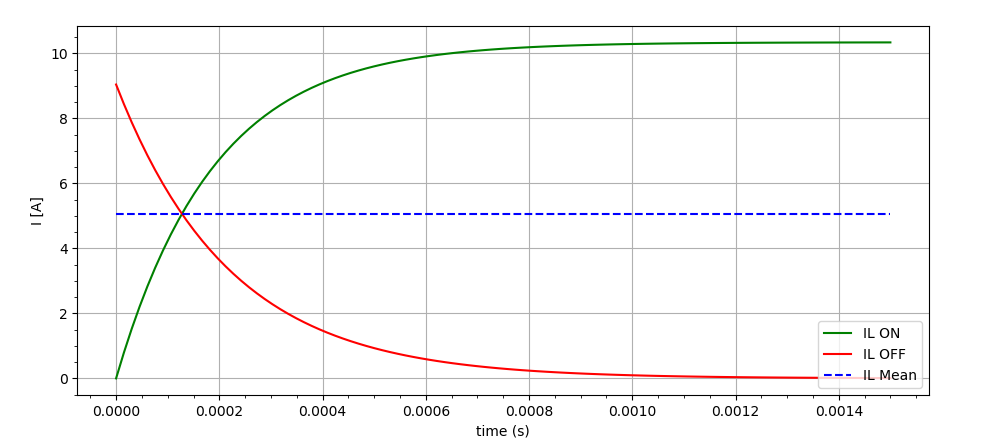
\includegraphics[width=0.8\linewidth]{ImagenesEjercicio-1/solgraficaIL}
	\caption{Solución gráfica de la corriente media en la bobina en régimen permanente.}
	\label{ej1:fig:ILmediagrafico}
\end{figure}

Conociendo la corriente media de la bobina, aproximando la tensión en cada estado como constante y teniendo en cuenta que la tensión media en los bornes de una inductancia debe ser nula en régimen permanente, se deduce que la forma de onda de $V_L$ será aproximadamente cuadrada, con una amplitud de $V_{max} = -V_{min} \approx V_D + \bar{I_L}R_2 = 6.47V$ observando la malla formada en la Figura (\ref{ej1:fig:circuito_off}). El ripple en la corriente $I_L$ será 

\begin{equation}
\Delta I_L = \frac{V_{max}}{L}\frac{D}{f_{sw}} = 245.1mA
\end{equation}

y el ripple en la tensión $V_L$ puede hallarse según la Ecuación (\ref{ej1:eq:VL_on}) como

\begin{equation}
\Delta V_L = \left[ V_2 - \bar{I_L} (R_{ds_{on}}+R_2) \right] \cdot (1-e^{-\frac{R_{ds_{on}} + R_2}{L}\frac{D}{f_{sw}}}) = 258mV
\end{equation}

Finalmente, la corriente en el diodo $I_{diodo}$ será igual a la corriente en la bobina cuando el MOSFET se encuentra apagado, y nula cuando el MOSFET se encuentra prendido, como se observa en la Figura (\ref{ej1:fig:idiodo_permanente}). La tensión $V_{ds}$ del MOSFET será igual a $13.3V$ durante el estado apagado como calculado en la sección anterior y $I_{L_{on}}(t) \cdot R_{ds_{on}} \approx \bar{I_L} \cdot R_{ds_{on}} = 827mV$ durante el estado encendido.

\begin{figure}[H]
	\centering
	\begin{minipage}{0.495\textwidth}
		\centering
		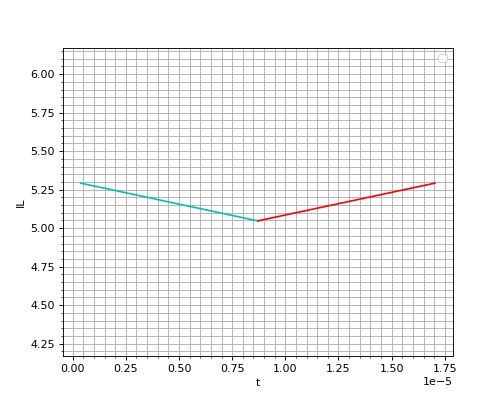
\includegraphics[width=\textwidth]{ImagenesEjercicio-1/IL_permanente} % first figure itself
		\caption{Corriente en la bobina en régimen permanente.}
		\label{ej1:fig:il_permanente}
	\end{minipage}\hfill
	\begin{minipage}{0.495\textwidth}
		\centering
		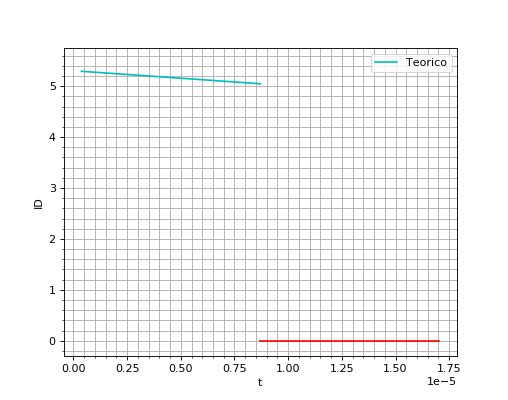
\includegraphics[width=\textwidth]{ImagenesEjercicio-1/ID_apagado_a_encendido} % second figure itself
		\caption{Corriente del diodo y $V_{ds}$ en régimen permanente.}
		\label{ej1:fig:idiodo_permanente}
	\end{minipage}
\end{figure}
Donde los colores simbolizan las distintas conmutaciones del MOS.
\subsubsection{Análisis de los Tiempos de Conmutación: Encendido}

Al encender el MOSFET con un escalón de tensión de $V_{GG} = 12V$, tomado en el borne izquierdo de $R_1$ y referido a masa, crece la corriente de gate $I_G$ rápidamente a un valor de $I_G = \frac{V_i}{R_1} = 0.12A$ para luego decrecer exponencialmente según (\ref{ej1:eq:ig_ton}). Al mismo tiempo, la tensión entre gate y source pasa de ser nula a crecer exponencialmente según (\ref{ej1:eq:vgs_ton}).

\begin{equation}
I_G(t) = \frac{V_{GG}}{R_1}e^{-\frac{t}{\tau_1}}
\label{ej1:eq:ig_ton}
\end{equation}

\begin{equation}
V_{gs}(t) = V_{GG}(1-e^{-\frac{t}{\tau_1}})
\label{ej1:eq:vgs_ton}
\end{equation}

Donde la constante de tiempo $\tau_1 = R_1 (C_{gs}+C_{gd_{1}}) = 75ns$ es regida por la capacidad de entrada del MOSFET compuesta por la capacitancia entre gate y source y la situada entre gate y drain, con un valor de $C_{gs}+C_{gd_{1}} = 750pF$ observado en la Figura (\ref{ej1:fig:cgd}). Cuando la tensión entre gate y source llega al valor de threshold $V_{gs_{th}} = 4V$ (proporcionada por la datasheet del IRF530) luego de un tiempo 
\begin{equation}
t_{d_{on}} = -\tau_1 ln\left( 1-\frac{V_{th}}{V_2} \right) = 30ns
\label{ej1:eq:tdon}
\end{equation}

según la Ecuación (\ref{ej1:eq:vgs_ton}), comienza a crecer la corriente de drain $I_{ds}$ con pendiente constante. Una vez que la corriente de drain $I_{ds}$ alcanza el valor medio de la corriente de la bobina $\bar{I_L}$, se observa en la Figura (\ref{ej1:fig:vgsio}) proporcionada por la datasheet del IRF530 que la tensión $V_{gs}$ será $V_{gs_{io}} = 5.5V$. Utilizando este valor y la Ecuación (\ref{ej1:eq:vgs_ton}) se obtiene que el tiempo de rise de la corriente de drain es

\begin{equation}
	t_{ri} = -\tau_1 ln\left( 1-\frac{V_{gs_{io}}}{V_2} \right) -t_{d_{on}} = 16ns
\label{ej1:eq:trise}
\end{equation}

La tensión $V_{ds}$ no disminuye hasta que la corriente $I_D$ no es lo suficientemente alta para que la corriente del diodo sea en consecuencia lo suficientemente baja para que este se polarice en inversa. Es cuando el diodo se polariza en inversa y no deja pasar corriente que la tensión entre sus bornes comienza a aumentar, lo que genera que la caída de tensión del MOSFET disminuya. A partir de este momento, se formará la zona de agotamiento del body layer en el transistor y la $V_{ds}$ comenzará a caer. La tensión $V_{gs} = V_{gs_{io}}$ y la corriente $I_G = \frac{V_{GG}-V_{gs_{io}}}{R_1} = 65mA$ se mantendrá constante mientras la capacitancia $C_{gd}$ se incrementa de $C_{gd_1}$ a $C_{gd_2}$ debido a la formación de la susodicha zona de agotamiento. Luego de un tiempo $t_{fv}$ en el que fluyó una carga de $\Delta Q = 7.3nC$ al gate del MOSFET, dato proporcionado de la datasheet del IRF530 visto en la Figura (\ref{ej1:fig:deltaq}), la tensión $V_{ds}$ alcanzará un valor $V_{ds} = V_{ds_{on}} = \bar{I_L} R_{ds_{on}} = 828mV$ utilizando el valor de $\bar{I_L}$ calculado en la Ecuación (\ref{ej1:eq:ilbar}). El tiempo transcurrido en esta transición puede calcularse teniendo en cuenta la corriente $I_G = \frac{V_2 - V_{gs_{io}}}{R_1}= 65mA$ obteniendo

\begin{equation}
	t_{fv} = \frac{R_1 \Delta Q}{V_2 - V_{gs_{io}}} = 112ns
	\label{ej1:eq:tfv}
\end{equation}

Finalmente, habiendo transicionado la capacitancia $C_{gd}$ de $C_{gd_1}$ a $C_{gd_2}$, se terminará de cargar el capacitor parásito de entrada del MOSFET según las Ecuaciones (\ref{ej1:eq:vgs_ton_2}) y (\ref{ej1:eq:ig_ton_2}).

\begin{equation}
V_{gs}(t) = V_{GG}(1-e^{-\frac{t}{\tau_2}})
\label{ej1:eq:vgs_ton_2}
\end{equation}

\begin{equation}
I_{G}(t) =  \frac{V_{GG}-V_{gs_{io}}}{R_1}e^{-\frac{t}{\tau_2}}
\label{ej1:eq:ig_ton_2}
\end{equation}

siendo $\tau_2 = R_1(C_{gs} + C_{gd_2}) = 115ns$ donde $C_{gs} + C_{gd_2} = 1150pF$ observado en la Figura (\ref{ej1:fig:cgd}). Se puede observar en las Figuras (\ref{ej1:fig:encendido_gate}) y (\ref{ej1:fig:encendido_drain}) el proceso entero de encendido descrito anteriormente.
\begin{multicols}{2}
\begin{figure}[H]
	\centering
	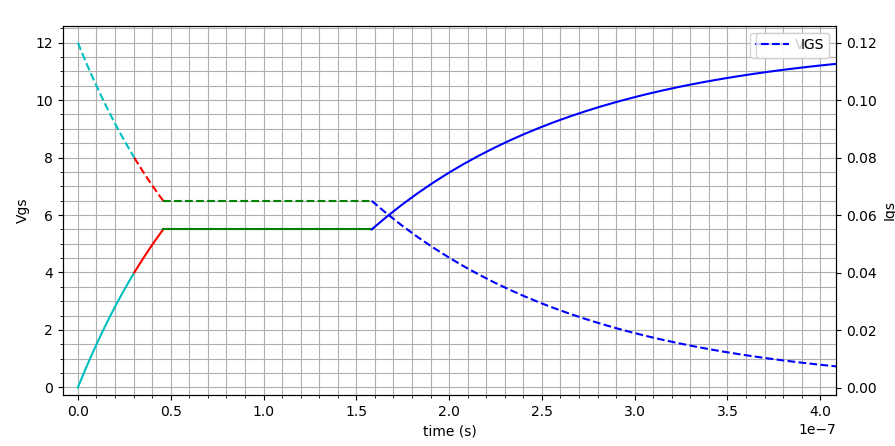
\includegraphics[width=\linewidth]{ImagenesEjercicio-1/encendido_gate}
	\caption{$V_{gs}$ e $I_G$ en el encendido del MOSFET.}
	\label{ej1:fig:encendido_gate}
\end{figure}

\begin{figure}[H]
	\centering
	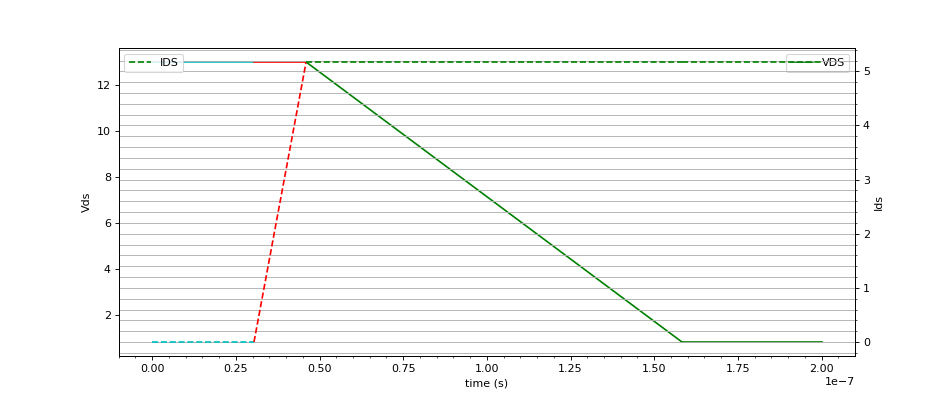
\includegraphics[width=\linewidth]{ImagenesEjercicio-1/encendido_drain}
	\caption{$V_{ds}$ e $I_D$ en el encendido del MOSFET.}
	\label{ej1:fig:encendido_drain}
\end{figure}
\end{multicols}
\begin{figure}[H]
	\centering
	\begin{minipage}{0.45\textwidth}
		\centering
		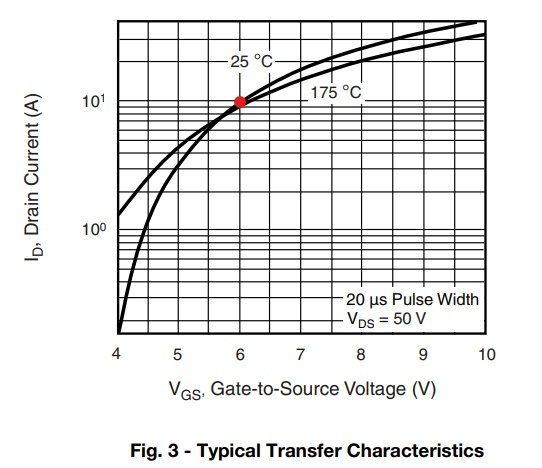
\includegraphics[width=\textwidth]{ImagenesEjercicio-1/Vgs-Id_LI} % first figure itself
		\caption{$V_{gs_{io}}$ de la datasheet del IRF530.}
		\label{ej1:fig:vgsio}
	\end{minipage}\hfill
	\begin{minipage}{0.45\textwidth}
		\centering
		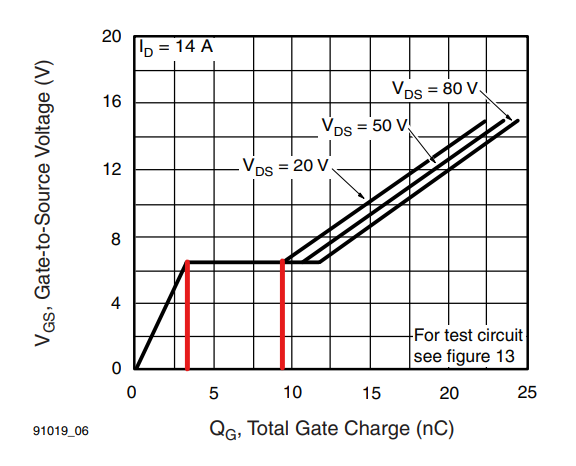
\includegraphics[width=\textwidth]{ImagenesEjercicio-1/deltaq} % second figure itself
		\caption{$\Delta Q$ en la transición de $C_{gd_1}$ a $C_{gs_2}$ de la datasheet del IRF530.}
		\label{ej1:fig:deltaq}
	\end{minipage}
\end{figure}

\begin{figure}[H]
	\centering
	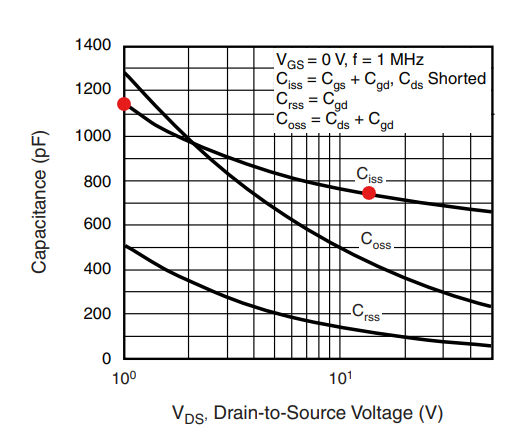
\includegraphics[width=0.4\linewidth]{ImagenesEjercicio-1/Vds-C}
	\caption{Capacitancia de entrada del MOSFET según la datasheet del IRF530 donde no ingresa carga al capacitor parásito $C_{gs}$ debido a la tensión constante $V_{gs}$.}
	\label{ej1:fig:cgd}
\end{figure}

\subsubsection{Análisis de los Tiempos de Conmutación: Apagado}

Al hacer nula la tensión $V_{GG}$ tomada a la izquierda del resistor $R_1$, comienza el apagado del MOSFET. La corriente $I_G$, medida como entrante al gate, se torna instantáneamente negativa con un valor de $I_G = \frac{0V-12V}{R_1} = -120mA$ a causa del descargado del capacitor parásito de entrada del MOSFET, compuesta por las capacitancias $C_{gs} + C_{ds}$. Este capacitor parásito se encontraba cargado debido al previo encendido del transistor, donde se asume que la tensión $V_{gs}$ alcanzó una tensión igual a $V_2 = 12V$.

Como tanto el apagado como el encendido del transistor poseen el mismo circuito, las constantes de tiempo $\tau_1$ y $\tau_2$ serán las mismas. Sin embargo, ahora estudiaremos la descarga del capacitor parásito de entrada.

En primer lugar, la tensión $V_{gs}$ cae según (\ref{ej1:eq:vgs_off_1}) hasta el valor $V_{gs_{io}} = 5.5V$ mientras que la corriente $I_G$ disminuye su valor en módulo según (\ref{ej1:eq:ig_off_1}) hasta $I_G = \frac{0V - V_{gs_{io}}}{R_1} = -55mA$ en un proceso que dura

\begin{equation}
t_{d_{off}} = -\tau_2 ln(\frac{V_{gs_{io}}}{V_2}) = 90ns
\label{ej1:eq:toff}
\end{equation}

\begin{equation}
V_{gs}(t) = V_2e^{-\frac{t}{\tau_2}}
\label{ej1:eq:vgs_off_1}
\end{equation}

\begin{equation}
I_{g}(t) = \frac{0V-V_2}{R_1} e^{-\frac{t}{\tau_2}}
\label{ej1:eq:ig_off_1}
\end{equation}

Luego, tanto la tensión $V_{gs}$ como la corriente $I_G$ se mantienen constantes por un tiempo igual a 

\begin{equation}
t_{rv} = \frac{R_1 \Delta Q}{V_{gs_{io}}} = 133ns
\label{ej1:eq:trv}
\end{equation}

con valores $5.5V$ y $\frac{0V-5.5V}{R_1} = -55mA$ respectivamente. Durante este tiempo la carga total egresada del gate del MOSFET será provista por el capacitor parasítico $C_{gd}$ el cual transicionará en este proceso de $C_{gd_2}$ a $C_{gd_1}$. Además, a lo largo de este tiempo $t_{rv}$, comenzará a crecer la tensión $V_{ds}$ hasta el valor de $V_{ds} = V_{ds_off} = 13.3V$ deducido anteriormente.

A partir de este momento, la corriente de drain disminuirá hasta cero en un tiempo

\begin{equation}
t_{fi} = -\tau_1 ln\left( \frac{V_{gs_{th}}}{V_{gs_{io}}} \right) = 24ns
\label{ej1:eq:tfi}
\end{equation}

mientras que la tensión $V_{gs}$ y corriente $I_G$ disminuirán exponencialmente hasta $V_{gs_{th}}$ y $\frac{0V-V_{gs_{th}}}{R_1}$ según (\ref{ej1:eq:vgs_off_2}) y (\ref{ej1:eq:ig_off_2}) para finalmente tender a cero.

\begin{equation}
V_{gs}(t) = V_{gs_{io}} e^{-\frac{t}{\tau_1}}
\label{ej1:eq:vgs_off_2}
\end{equation}

\begin{equation}
I_{G}(t) = \frac{0V-V_{gs_{io}}}{R_1} e^{-\frac{t}{\tau_1}}
\label{ej1:eq:ig_off_2}
\end{equation}

\subsection{Circuito en la Simulación y Diferencias con los Cálculos Teóricos}

Se realizaron las simulaciones para este circuito utilizando el software \textit{LTSpice} % y el lenguaje de programación \textit{Python} para graficar las simulaciones sobre las curvas teóricas. Las configuraciones del %Se realizaron las simulaciones para este circuito utilizando el software \textit{LTSpiceXVII} y el lenguaje de programación \textit{Python} para graficar las simulaciones sobre las curvas teóricas. Las configuraciones del software se detallan en la Figura (\ref{ej1:fig:spice_specs}).
%
%\begin{figure}[H]
%	\centering
%	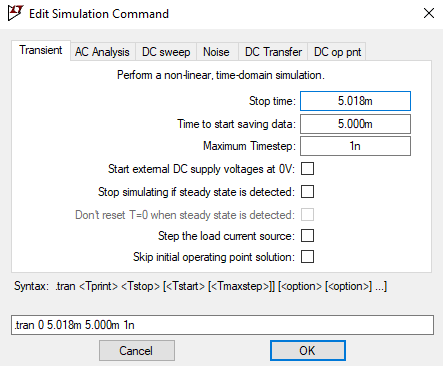
\includegraphics[width=0.4\linewidth]{ImagenesEjercicio-1/spice_specs}
%	\caption{Configuración para la simulación.}
%	\label{ej1:fig:spice_specs}
%\end{figure}

\subsubsection{Encendido del MOSFET}

Se puede observar que cuando el MOSFET es encendido, aparece en la simulación en la curva de $V_{gs}$ un pequeño sobrepico de tensión por encima de $V_{gs_{io}}$. Esto se debe a que el diodo, previamente polarizado en directa, debe evacuar los portadores de carga de la zona de drift y luego formar la zona de vaciamiento para lograr polarizarse en inversa. Esto esencialmente genera un gran pico de corriente en sentido contrario al del funcionamiento normal del diodo. Este pico de corriente, denominado $I_{rr}$ o reverse recovery current, genera que la corriente de drain $I_D$ del MOSFET aumente hasta $I_D = I_o+I_{rr}$ en vez de hasta $I_o$. Esto a su vez genera que la tensión $V_{gs}$ aumente por encima de $V_{gs_{io}}$. Una vez que la corriente de recovery del diodo se acaba, la tensión $V_{gs}$ y $V_{ds}$ caen abruptamente a los valores ideales.

Otra diferencia con lo calculado surge a raíz de que en los cálculos teóricos no se consideró el driver totem-pole del transistor que demanda tanto en el estado encendido como en el apagado una caída de máxima de $V_{ce_{sat}}$ a causa de la juntura colector emisor de los transistores bipolares. Es por esto que en la Figura (\ref{ej1:fig:sim_encendido_gate}) se observa que la curva simulada de $V_{gs}$ no comienza en $0V$ ni termina en $12V$, sino en $\approx 0.6V$ y $\approx 11.4V$ respectivamente.

Tanto en $V_{ds}$ como $I_D$ se observan diferencias en las formas de las curvas, sin embargo estas se deben a la linealización de los cálculos teóricos.

Por otro lado se puede ver que existen diferencias entre la curva teórica de la corriente de Gate y la simulación, esto se debe a el totem-pole  el cual cambia la forma de onda de un escalón a la observada en el gráfico \ref{ej1:fig:sim_encendido_gate_i}, si en vez del totem-pole se utilizase una fuente ideal de tensión las curvas corresponderían.

\begin{figure}
	\centering
	\begin{minipage}{0.5\textwidth}
		\centering
		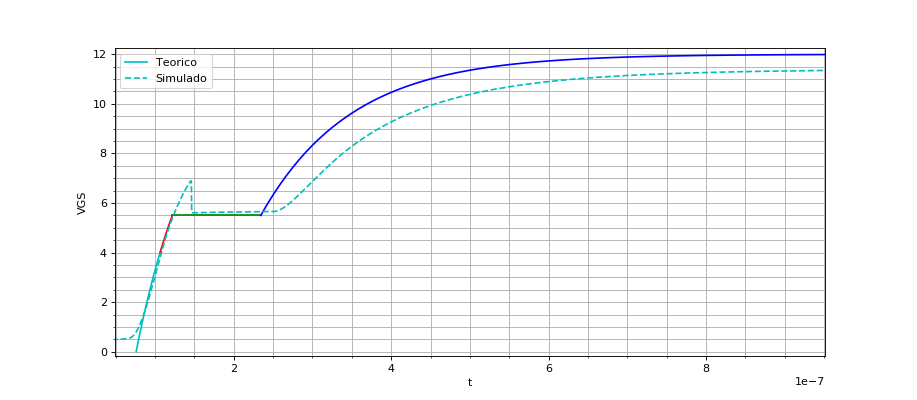
\includegraphics[width=1.1\textwidth]{ImagenesEjercicio-1/sim_encendido_gate} % first figure itself
		\caption{Comparación $V_{gs}$ entre simulado y calculado.}
		\label{ej1:fig:sim_encendido_gate}
	\end{minipage}\hfill
	\begin{minipage}{0.5\textwidth}
		\centering
		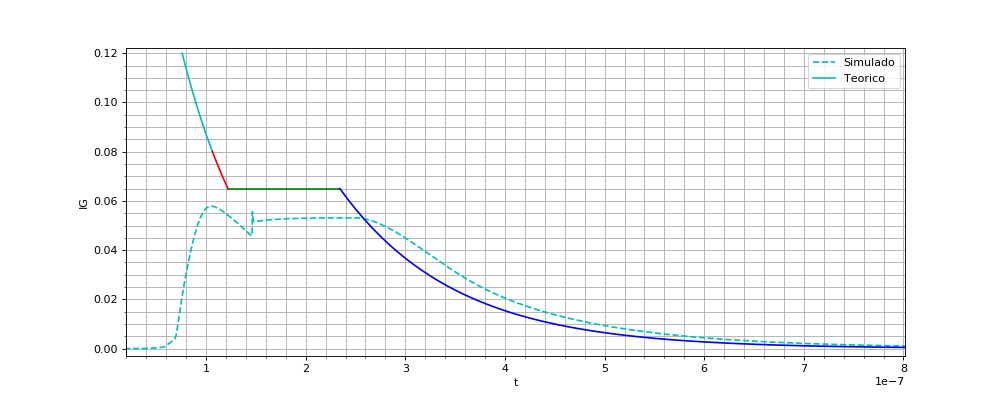
\includegraphics[width=1.1\textwidth]{ImagenesEjercicio-1/sim_encendido_gate_i} % second figure itself
		\caption{Comparación $I_{G}$ entre simulado y calculado.}
		\label{ej1:fig:sim_encendido_gate_i}
	\end{minipage}
\end{figure}

\begin{figure}
	\centering
	\begin{minipage}{0.5\textwidth}
		\centering
		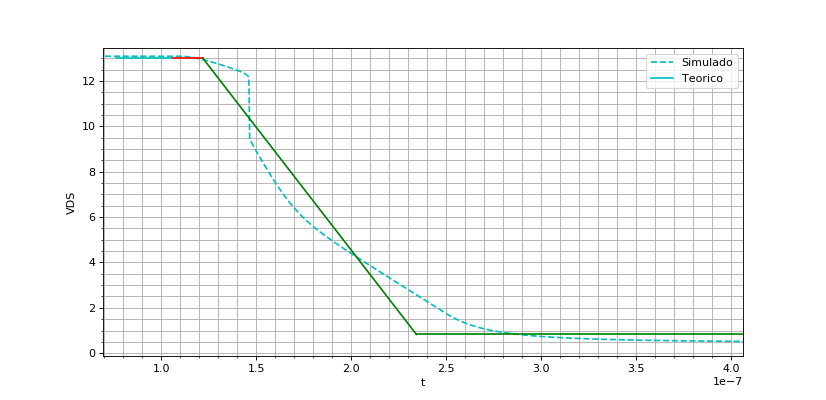
\includegraphics[width=1.1\textwidth]{ImagenesEjercicio-1/sim_encendido_drain} % first figure itself
		\caption{Comparación $V_{ds}$ entre simulado y calculado.}
		\label{ej1:fig:sim_encendido_drain}
	\end{minipage}\hfill
	\begin{minipage}{0.5\textwidth}
		\centering
		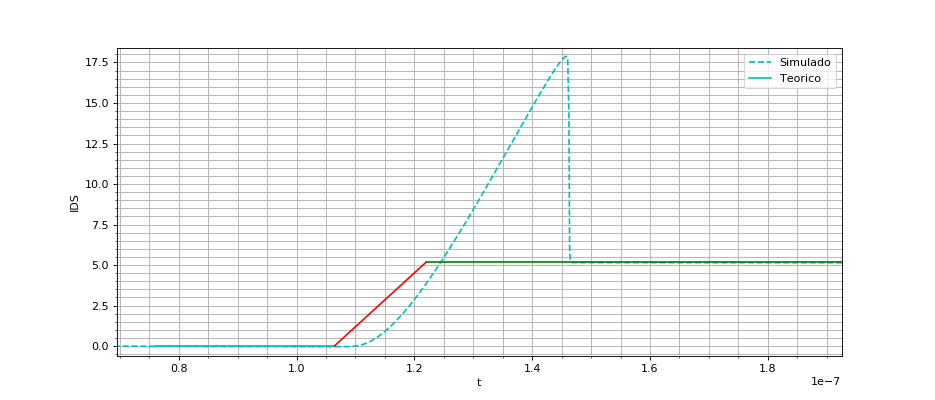
\includegraphics[width=1.1\textwidth]{ImagenesEjercicio-1/sim_encendido_drain_i} % second figure itself
		\caption{Comparación $I_{D}$ entre simulado y calculado.}
		\label{ej1:fig:sim_encendido_drain_i}
	\end{minipage}
\end{figure}



\subsubsection{Apagado del MOSFET}

Para el apagado del MOSFET se puede observar en la Figura (\ref{ej1:fig:sim_apagado_gate}) y en consecuencia la Figura (\ref{ej1:fig:sim_apagado_gate_i}) la caída $V_{ce_{sat}}$ a causa del totem pole discutido en la sección anterior.

Solamente se observan además de esto ligeras diferencias causadas por la linealización de las curva $V_{ds}$ en los calculos teóricos.

\begin{figure}
	\centering
	\begin{minipage}{0.5\textwidth}
		\centering
		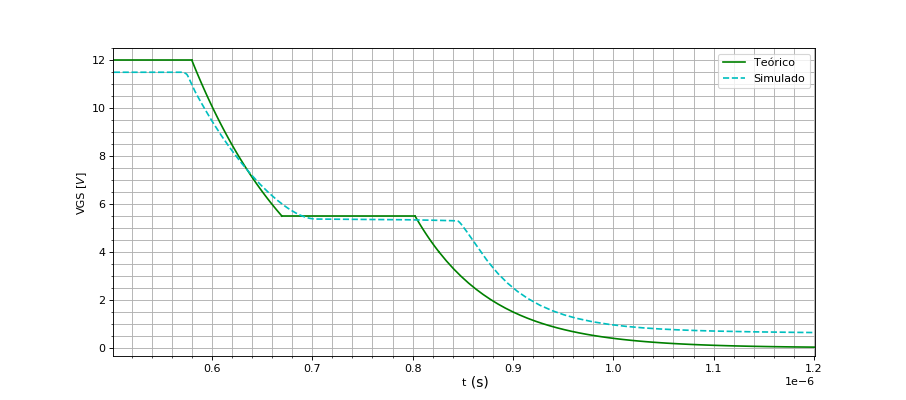
\includegraphics[width=1.1\textwidth]{ImagenesEjercicio-1/sim_apagado_gate} % first figure itself
		\caption{Comparación $V_{gs}$ entre simulado y calculado en el apagado.}
		\label{ej1:fig:sim_apagado_gate}
	\end{minipage}\hfill
	\begin{minipage}{0.5\textwidth}
		\centering
		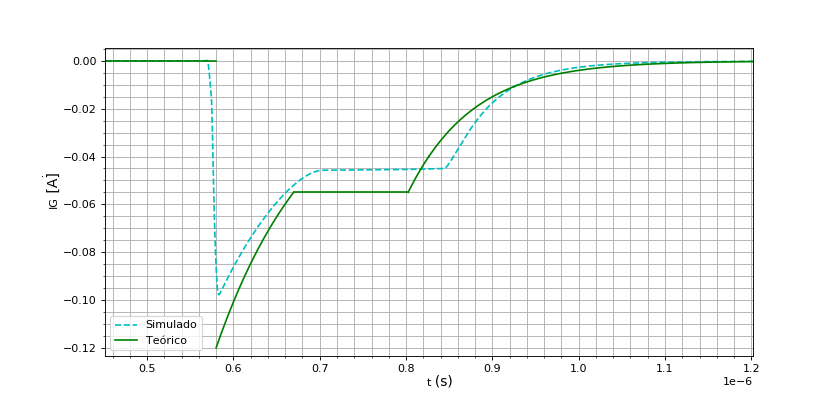
\includegraphics[width=1.1\textwidth]{ImagenesEjercicio-1/sim_apagado_gate_i} % second figure itself
		\caption{Comparación $I_{G}$ entre simulado y calculado en el apagado.}
		\label{ej1:fig:sim_apagado_gate_i}
	\end{minipage}
\end{figure}
\begin{figure}
	\centering
	\begin{minipage}{0.5\textwidth}
		\centering
		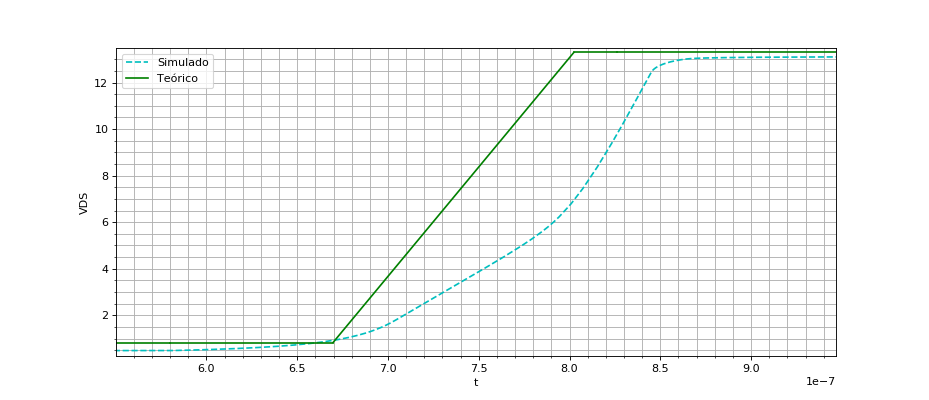
\includegraphics[width=1.1\textwidth]{ImagenesEjercicio-1/sim_apagado_drain} % first figure itself
		\caption{Comparación $V_{ds}$ entre simulado y calculado en el apagado.}
		\label{ej1:fig:sim_apagado_drain}
	\end{minipage}\hfill
	\begin{minipage}{0.5\textwidth}
		\centering
		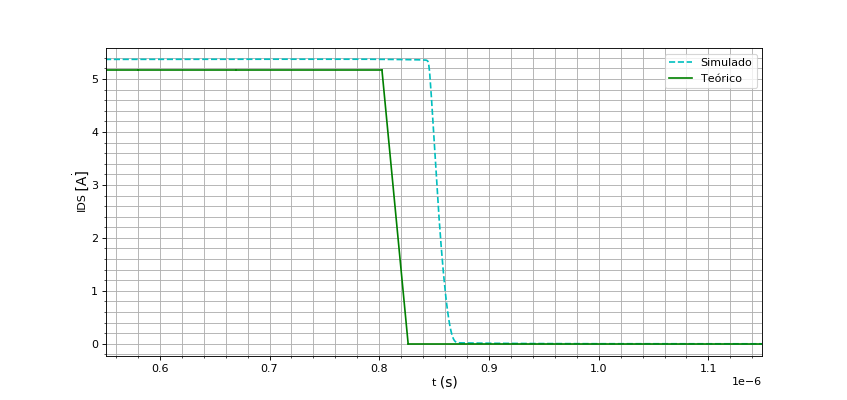
\includegraphics[width=1.1\textwidth]{ImagenesEjercicio-1/sim_apagado_drain_i} % second figure itself
		\caption{Comparación $I_{D}$ entre simulado y calculado en el apagado.}
		\label{ej1:fig:sim_apagado_drain_i}
	\end{minipage}
\end{figure}

\subsubsection{Corriente de la Bobina y Diodo en Régimen Permanente}

Para el caso de la corriente en la bobina, se observa en la Figura (\ref{ej1:fig:il_permanente_sum}) que el ripple de corriente calculado es igual que el ripple de corriente en la simulación. Sin embargo, existe una diferencia de $90mA$ (error porcentual de un $1.74\%$) en la corriente media de la bobina.

\begin{figure}[H]
	\centering
	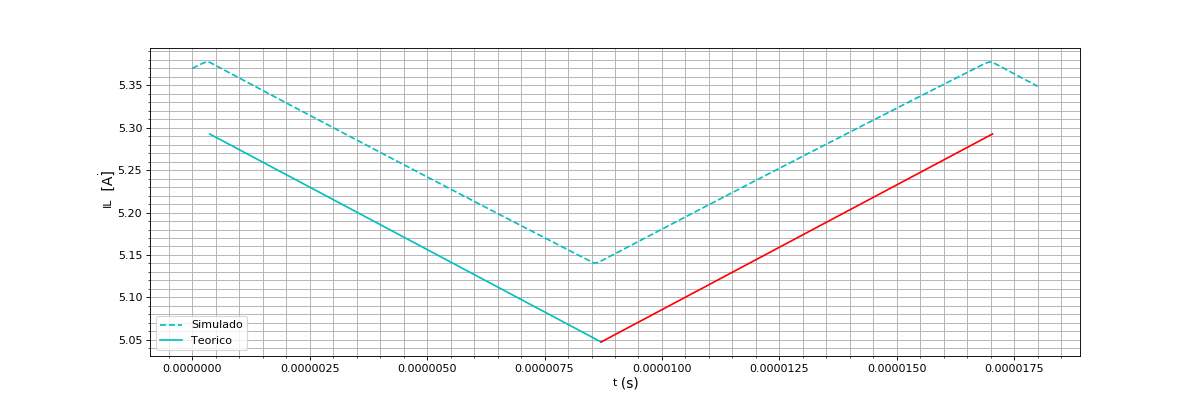
\includegraphics[width=0.8\linewidth]{ImagenesEjercicio-1/il_permanente_sim}
	\caption{Comparación entre $I_L$ calculado y simulado en régimen permanente.}
	\label{ej1:fig:il_permanente_sum}
\end{figure}
Mientras tanto en la corriente del Diodo, el mismo seguirá a la corriente de la bobina en el semiciclo donde la llave se encuentra abierta, y luego irá a cero cuando la llave se encuentre cerrada.
\begin{figure}[H]
	\centering
	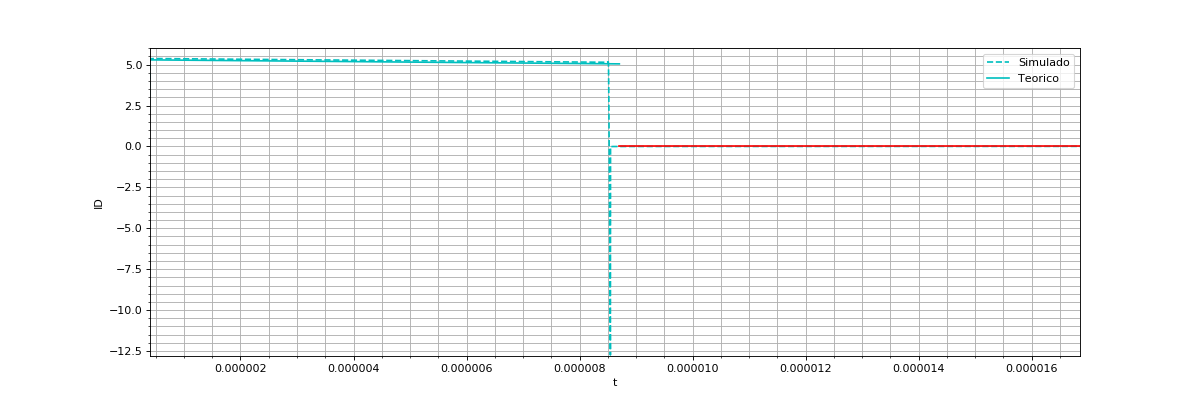
\includegraphics[width=0.8\linewidth]{ImagenesEjercicio-1/id_permanente_sim}
	\caption{Comparación entre $I_D$ calculado y simulado en régimen permanente.}
	\label{ej1:fig:id_permanente_sum}
\end{figure}
Se puede observar que hay un gran sobre pico de corriente cuando el diodo conmuta de directa a inversa, esto se debe a la corriente de reverse recovery.
Ademas si se hace un detalle en la imagen (\ref{ej1:fig:id_permanente_sum}) se puede observar que son paralelas las corrientes (\ref{ej1:fig:id_permanente_sum_det}), al igual el pequeño offset que existe el cual fue explicado anteriormente.
\begin{figure}[H]
	\centering
	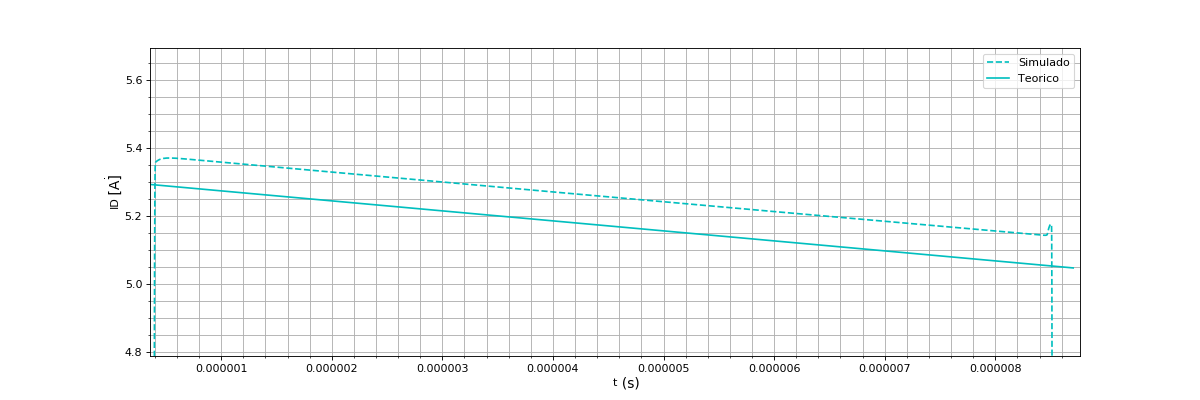
\includegraphics[width=0.8\linewidth]{ImagenesEjercicio-1/id_permanente_sim_det}
	\caption{Comparación entre $I_D$ calculado y simulado en régimen permanente detalle.}
	\label{ej1:fig:id_permanente_sum_det}
\end{figure}

\subsubsection{Comparación con los Tiempos de Conmutación Calculados}


A continuación se observa un cuadro comparativo de las los tiempos calculados y los medidos en simulación.
\begin{table}[H]
\centering
\begin{tabular}{@{}lllllll@{}}
\toprule
 & $t_{d_{on}}$ & $t_{ri}$ & $t_{fv}$ & $t_{d_{off}}$ & $t_{rv}$ & $t_{fi}$ \\ \midrule
Calculado & $30ns$ & $16ns$ & $112ns$ & $90ns$ & $133ns$ & $24ns$ \\
Simulado & $41ns$ & $15ns$ & $107ns$ & $122ns$ & $138ns$ & $28ns$ \\
Error Porcentual & $-26.8\%$ & $6.66\%$ & $4.67\%$ & $-26.2\%$ & $-3.62\%$ & $-14.3\%$ \\ \bottomrule
\end{tabular}
\caption{Comparación entre tiempos calculados y simulados.}
\end{table}
Se puede apreciar que no hay un error significativo en los cálculos y lo simulado.
%\subsection{Circuito en la Práctica}

\subsection{Conclusiones}
Se calcularon y midieron los tiempos de conmutación al igual que las curvas de tensión y corriente del MOSFET al igual que la bobina y diodo, obteniendo resultados los cuales se corresponden lo simulado con lo teórico en gran medida. Se pudieron observar las curvas de conmutación del MOSFET con todas sus particularidades y explicar las diferencias entre lo teórico y simulado.
%\end{document}
